%*******************************************************************************
%****************************** Fifth Chapter *********************************
%*******************************************************************************

\chapter{Characterisation of III-Nitride Nanobeam Cavities}

\ifpdf
    \graphicspath{{Chapter2/Figs/Raster/}{Chapter2/Figs/PDF/}{Chapter2/Figs/}}
\else
    \graphicspath{{Chapter2/Figs/Vector/}{Chapter2/Figs/}}
\fi


\section[Background]{Background}
In chapter \ref{Microdisk Chapter} we have touched upon some challenges in the fabrication of III-nitride cavities due to the properties of III-nitride materials, as well as microscopy-based methods to characterise the structural and compositional properties of these cavities. In this chapter we extend these methods and apply them to 1-D PCCs, or nanobeam cavities. As discussed in section \ref{nanobeam section}, nanobeam cavities provide several advantages over other cavity geometries, namely ease of fabrication relative to 3-D PCC structures and their ability to realise high Q-factor and low effective modal volumes required for applications such as low-threshold lasing. Relative to microdisk cavities, nanobeam cavities require several additional fabrication steps due to their complex geometry and thus are more susceptible to fabrication issues such as non-uniform patterning and incomplete undercutting. This chapter will present the work done on harnessing microscopy techniques in order to characterise the fabrication of III-nitride nanobeam cavities.

\section{Nanobeam Fabrication}
\label{nbfab}
The nanobeam cavities studied in this work were fabricated by Dr. Nan Niu and Danqing Wang in the Hu group at Harvard University. The samples are similar to those described in section \label{microdisk samples}, in that they contain InGaN active layers in a GaN membrane, an InGaN SSL for PEC undercutting and an AlGaN layer to prevent the PEC etching from affecting the InGaN active region. The fabrication flow for the devices is shown in Fig.\ref{nanobeamfab}.\\
The fabrication scheme utilises e-beam lithography to pattern the shape of the nanobeam. XR-1541(XR) e-beam resist is spun on to the surface of the wafer and is patterned to define the nanobeam and circular pads. The resist is then removed, remaining only in the patterned areas and acting as a mask for the inductively coupled plasma (ICP) dry etch. This dry etch allows access to the InGaN SSL which is selectively undercut by the PEC etching method described in section \ref{microdisk fab section}.

\begin{figure}[h]
	\centering
	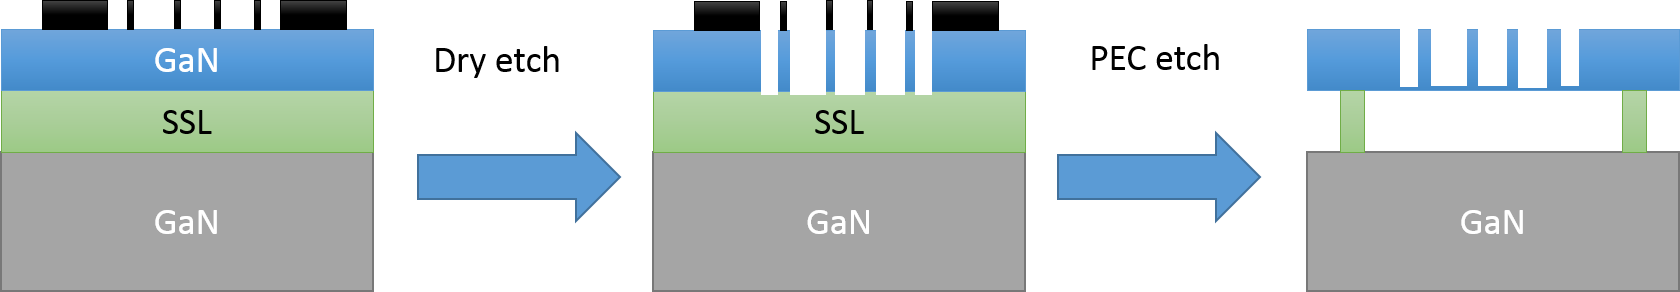
\includegraphics[width=1\textwidth]{Figs/Ch5/nanobeamfab.png}
	\caption {Nanobeam cavity workflow.}
	\label{nanobeamfab}
\end{figure}
\FloatBarrier 

Top and side view SEM images of a fabricated nanobeam produced from this process are shown in Fig.\ref{nb}.

\begin{figure}[h]
	\centering
	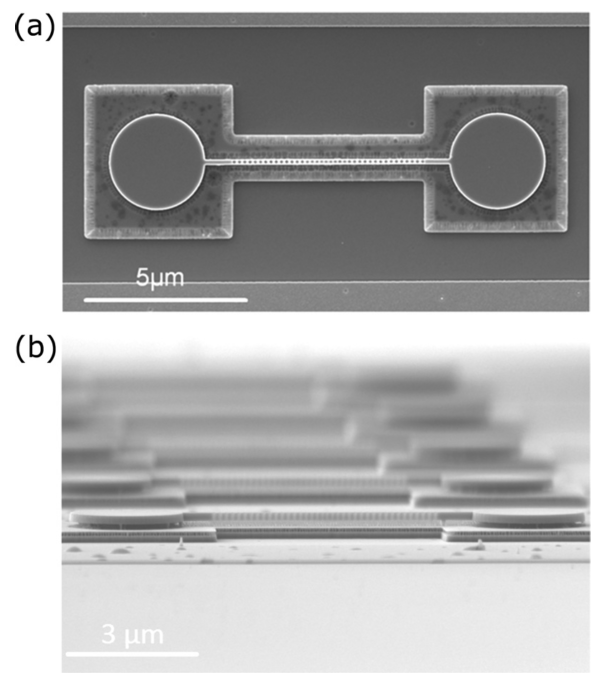
\includegraphics[width=0.6\textwidth]{Figs/Ch5/nb.png}
	\caption {a) Top-view and b) side-view of the suspended nanobeam cavities. Reproduced from \cite{Niu2015}.}
	\label{nb}
\end{figure}
\FloatBarrier 

\section{Experimental}

Fig.\ref{nb}.a. shows that the nanobeams are extremely narrow in one direction (approximately 125 nm), thus making them electron transparent to a 200 kV electron beam \cite{Rao2010}. This introduces an interesting problem in terms of TEM specimen problem: on the one hand the nanobeams are already at the required thickness and thus require no additional thinning once extracted. However, as seen with the microdisks in section \ref{udiskFIBsection} suspended structures are extremely sensitive to ion-beam damage which is required for sample lift-out in FIB/SEM dual beam equipment. Furthemore, the standard method of using protective Pt can not be applied here, as this would cover the entirety of the specimen and hinder TEM/STEM imaging. This section will cover FIB techniques used to extract nanobeams, and the TEM analysis performed on these samples.

\subsection{Nanobeam Lift-out}
In this section we will present the work performed on nanobeam cavities using standard FIB lift-out techniques.\\
Initial attempts to lift-out nanobeam cavities using standard dual-beam techniques were unsuccessful for several reasons. Firstly, the small width of the nanobeams relative to the Omniprobe provide a difficult target to reach accurately using the probe. Furthermore, even after successfully welding the nanobeam to the Omniprobe using Pt, the fragility of the nanobeams renders the lifting out of a whole nanobeam intact rather difficult, as shown in Fig.\ref{brokennb}.

\begin{figure}[h]
	\centering
	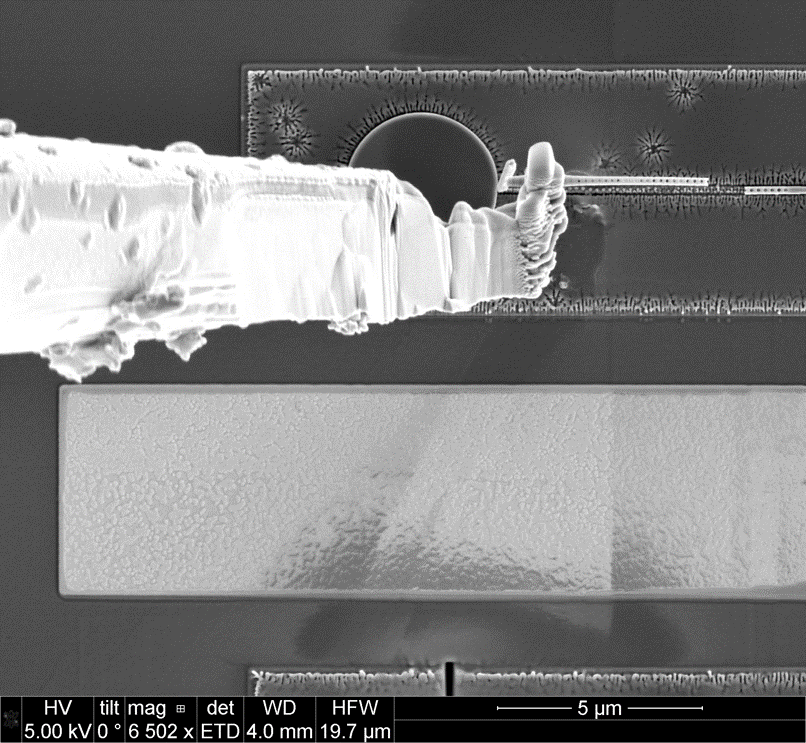
\includegraphics[width=0.5\textwidth]{Figs/Ch5/brokennb.png}
	\caption {SEM image of the Omniprobe attached to a broken nanobeam cavity.}
	\label{brokennb}
\end{figure}
\FloatBarrier 

An additional challenge was encountered when attaching the sample to the TEM grid. In the process of welding the nanobeam, the Pt used would cover the entire sample despite being targeted in a minute region, as shown in Fig.\ref{nbcovered}. The image shows that the etched holes are no longer visible, as such this type of sample preparation is unsatisfactory for TEM analysis.

\begin{figure}[h]
	\centering
	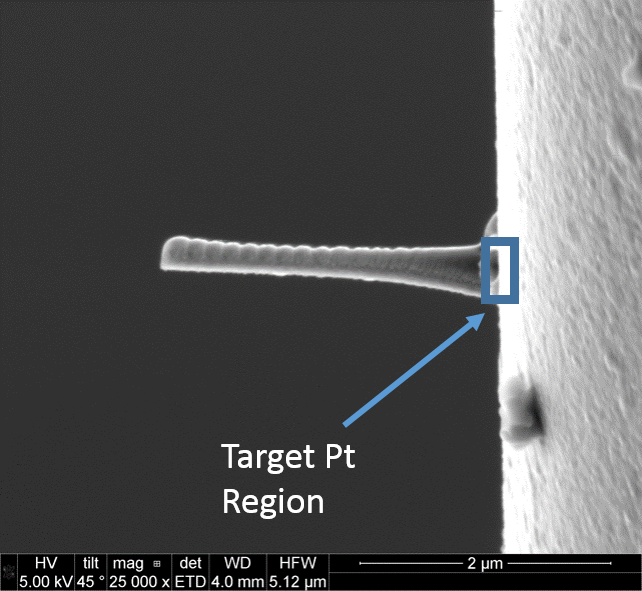
\includegraphics[width=0.4\textwidth]{Figs/Ch5/nbcovered.png}
	\caption {SEM image of a nanobeam attached to a TEM grid covered in platinum.}
	\label{nbcovered}
\end{figure}
\FloatBarrier 

In order to attempt to mitigate the negative effect of the Pt, carbon was used as a welding material to join the nanobeam to the TEM grid instead, as it was anticipated that the low atomic number of C relative to Pt would result in lower contrast from the carbon layer in STEM-HAADF. Fig.\ref{carbonnb} shows STEM-HAADF images of the carbon covered nanobeam cavity. Despite the presence of carbon which can be seen on the nanobeam, Fig.\ref{carbonnb}.b. the contrast from the InGaN active region can be observed.

\begin{figure}[h]
	\hspace*{2cm}
	\begin{subfigure}[b]{0.35\textwidth}
		\centering
		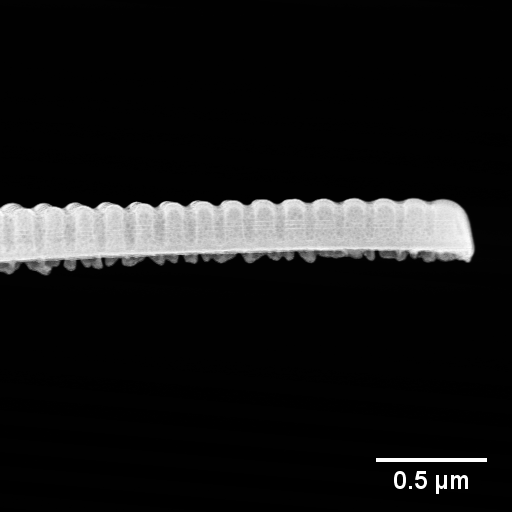
\includegraphics[width=1\linewidth]{Figs/Ch5/nb2}
		\caption{}
		
	\end{subfigure}%
	\hspace*{2cm}
	\begin{subfigure}[b]{0.35\textwidth}
		\centering
		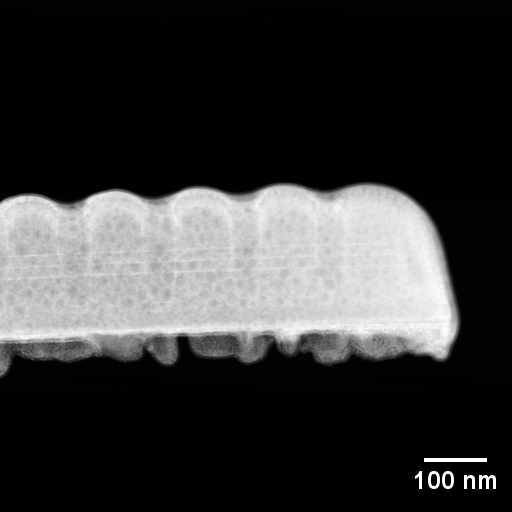
\includegraphics[width=1\linewidth]{Figs/Ch5/nb1}
		\caption{}
	\end{subfigure}%
	
	\caption{STEM-HAADF images of a carbon covered nanobeam.}
	\label{carbonnb}
\end{figure}
\FloatBarrier

Fig.\ref{carbonnb} shows the holes in the nanobeam cavity are incompletely etched through, indicating the dry etch step described in section \ref{nbfab} may have been terminated prematurely. 
